% Figure: references under location-based and content-addressed persistence.
% Standalone TikZ source; build.sh compiles the file to version-pinning.pdf.
% Positions use explicit anchors, because the positioning keys reset the anchor.
\documentclass[tikz,border=2pt]{standalone}
\usetikzlibrary{arrows.meta,calc}

\definecolor{ink}{HTML}{0B0B0B}
\definecolor{inksoft}{HTML}{52514E}
\definecolor{muted}{HTML}{898781}
\definecolor{mutablefill}{HTML}{F0EFEC}
\definecolor{immutablefill}{HTML}{CDE2FB}
\definecolor{immutableborder}{HTML}{1C5CAB}

\begin{document}
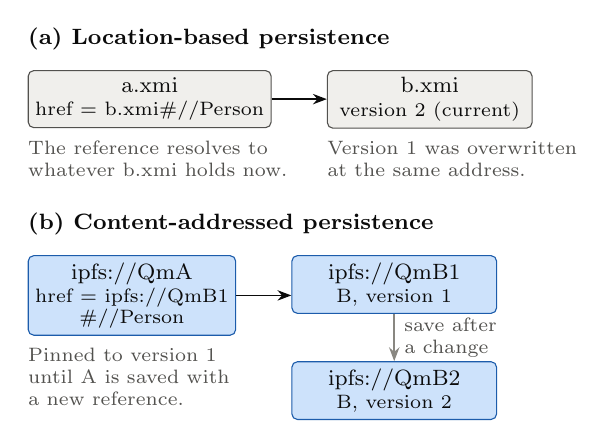
\begin{tikzpicture}[
  font=\footnotesize,
  >={Stealth[length=5pt]},
  box/.style={draw=inksoft, rounded corners=2pt, minimum height=7mm, minimum width=26mm, inner sep=2.5pt, align=center, text=ink, anchor=north west},
  mutable/.style={box, fill=mutablefill},
  immutable/.style={box, fill=immutablefill, draw=immutableborder},
  ref/.style={->, draw=ink, line width=0.6pt},
  change/.style={->, draw=muted, line width=0.6pt},
  paneltitle/.style={font=\footnotesize\bfseries, anchor=north west, text=ink, inner sep=0pt},
  note/.style={font=\scriptsize, text=inksoft, align=left, anchor=north west, inner sep=0pt}
]
\def\gap{7mm}

% (a) Location-based persistence
\node[paneltitle] (ta) at (0,0) {(a) Location-based persistence};
\node[mutable] (a) at ($(ta.south west)+(0,-2.5mm)$) {a.xmi\\[-1pt]\scriptsize href = b.xmi\#//Person};
\node[mutable] (b) at ($(a.north east)+(\gap,0)$) {b.xmi\\[-1pt]\scriptsize version 2 (current)};
\draw[ref] (a.east) -- (a.east-|b.west);
\node[note] (noteA) at ($(a.south west)+(0,-1.5mm)$) {The reference resolves to\\whatever b.xmi holds now.};
\node[note] (noteB) at ($(b.south west)+(0,-1.5mm)$) {Version 1 was overwritten\\at the same address.};

% (b) Content-addressed persistence
\node[paneltitle] (tb) at ($(noteA.south west)+(0,-4.5mm)$) {(b) Content-addressed persistence};
\node[immutable] (A) at ($(tb.south west)+(0,-2.5mm)$) {ipfs://QmA\\[-1pt]\scriptsize href = ipfs://QmB1\\[-2pt]\scriptsize \#//Person};
\node[immutable] (B1) at ($(A.north east)+(\gap,0)$) {ipfs://QmB1\\[-1pt]\scriptsize B, version 1};
\node[immutable] (B2) at ($(B1.south west)+(0,-6mm)$) {ipfs://QmB2\\[-1pt]\scriptsize B, version 2};
\draw[ref] (A.east) -- (A.east-|B1.west);
\draw[change] (B1.south) -- node[right, font=\scriptsize, text=inksoft, align=left] {save after\\a change} (B2.north);
\node[note] at ($(A.south west)+(0,-1.5mm)$) {Pinned to version 1\\until A is saved with\\a new reference.};

\end{tikzpicture}
\end{document}
